\documentclass{article}

\usepackage[total={7.5in, 10in}]{geometry}
\usepackage[polish]{babel}
\usepackage{polski}
\usepackage{titlesec}
\usepackage[hidelinks]{hyperref}
\usepackage{float}
\usepackage{amsmath}
\usepackage{amsfonts}
\usepackage{caption}
\usepackage{graphicx}
\usepackage{subfig}

\newcommand{\tableimg}[3]{
    \begin{table}[H]
        \centering
        \captionsetup{font=small, skip=2pt}
        \caption{#2}
        \includegraphics[#3]{#1}
    \end{table}
}

\newcommand{\image}[3]{
    \begin{figure}[H]
        \centering
        \captionsetup{font=small, skip=2pt}
        \includegraphics[#3]{#1}
        \caption{#2}
    \end{figure}
}

% \doubleimage{<img_1>}{<img_2>}{<caption>}{<img_1_caption>}{<img_2_caption>}{<img_1_options>}{<img_2_options>}
\newcommand{\doubleimage}[7]{
    \begin{figure}[H]
        \centering
        \captionsetup{font=small, skip=2pt}
        \subfloat[#4]{\includegraphics[#6]{#1}}
        \hspace{1cm}
        \subfloat[#5]{\includegraphics[#7]{#2}}
        \caption{#3}
    \end{figure}
}

% TYLKO NUMERY!! B12 -> 12, B21 -> 21
\newcommand{\transkodery}[1]{
    \doubleimage{images/transkoder_b#1}{images/transkoder_b#1_box}{Transkoder dla bitu B#1}
    {Schemat transkodera}{Podukład}{scale=0.5}{scale=0.8}
}

\begin{document}
    \begin{titlepage}
        \vspace*{\fill}
        \begin{center}
            \textbf{
                \Huge TECHNIKA CYFROWA \\ Ćwiczenie nr. 2\\ Czterobitowy układ TIMER\\ \bigskip
                \Large Antoni Kucharski, Maciej Wilewski, Dawid Mularczyk, Kamil Lesiński
                }
        \end{center}
        \vspace*{\fill}
    \end{titlepage}

    \tableofcontents
    \pagebreak

    \section{Temat ćwiczenia}
    Za pomocą dowolnych przerzutników i bramek logicznych należało zaprojektować czterobitowy układ TIMER odmierzający
    ustawiany za pomocą przełączników czas w granicach od 0 do 15. Układ powinien rozpocząć odliczanie po wciśnięciu przycisku
    START, a gdy czas dojdzie do zera --- powinien się włączyć alarm w postaci diody LED. Ponowne wciśnięcie przycisku
    START ma uruchomić odliczanie po raz kolejny.

    \section{Opis rozwiązania}
    Układ który rozwiąże zadanie będzie składał się z:
    \begin{itemize}
        \item Czterech przełączników służących do ustawiania liczby od 0 do 15 włącznie, od której układ ma zacząć odliczanie 
        (liczbę reprezentujemy binarnie, stąd 4 przełączniki --- każdy reprezentuje jeden bit),
        \item Dwóch wyświetlaczy siedmiosegmentowych,
        \item Transkodera liczby binarnej na dziesiętną,
        \item Przełącznika modulującego tryb układu (TIME\_SET) \begin{itemize}
            \item Tryb odliczania: układ odlicza czas w dół od ustalonej wartości do zera
            \item Tryb ustawiania liczby: ustawiamy wspomnianymi wyżej przełącznikami liczbę, i widzimy ją na wyświetlaczach. Funkcja odliczania jest zablokowana.
            W poprzednim trybie można również ustawiać liczbę, lecz układ zacząłby od razu odliczanie.
        \end{itemize}
        \item Przycisku START uruchamiającego układ (korzystamy głównie gdy licznik doliczy się do zera, bo przełącznik TIME\_SET również może rozpocząć odliczanie).
        \item Licznika zbudowanego z przerzutników typu D
        \item Diody LED
    \end{itemize}
    Układ zasilany jest źródłem prądu zmiennego. Przełącznik TIME\_SET umożliwia uruchomienie programu, natomiast przełącznik
    start powoduje zrestartowanie odliczania. Odbywa się ono za pomocą przerzutników typu D. Podłączone są one do siedmiosegmentowych
    wyświetlaczy które pokazują odpowiednią liczbę. Przy pomocy tabel Karnaugh wyprowadzone zostały funkcje logiczne transkodera liczby binarnej na dziesiętną.

    \section{Licznik}
    Timer składa się z określonej liczby przerzutników (4) typu D. Pierwszy z nich jest podłączony do źródła prądu zmiennego. 


    \subsection{Przerzutnik typu D}
    Przerzutnik typu D jest jednym z podstawowych elementów w elektronice cyfrowej. Jest to dwustanowy układ logiczny, 
    który przechowuje jedną bitową wartość. Ma dwa wejścia: dane (D) i sygnał zegarowy (CLK), oraz dwa wyjścia: stan(Q)
    i stan sprzężony (Q'). 
    \begin{figure}[H]
        \centering
        \captionsetup{font=small, skip=2pt}
        \caption{Schemat przerzutnika}
        %\includegraphics{images/D_FF.png}
    \end{figure} 

    \subsection{Dzielenie częstotliwości przez 2}
    Przez sprzężenie zwrotne wyjścia z Q do wejścia D, impulsy wyjściowe na Q mają częstotliwość połowy częstotliwości
    zegara wejściowego.
    
    \image{images/czestotliwosc_na_2}{Zastosowanie przerzutnika typu D do dwukrotnego zmniejszenia częstotliwości sygnału zegarowego}{scale=0.5}

    \subsection{Licznik złożony z czterech przerzutników}
    Użyty przez nas licznik jest asynchroniczny. Każdy z przerzutników otrzymuje sygnał zegarowy o innej częstotliwości
    (pierwszy --- częstotliwość źródła, każdy kolejny --- połowę częstotliwości poprzedniego).
    \image{images/licznik_analizator}{Działanie licznika złożonego z czterech przerzutników typu D}{scale=0.5}
    Z analizatora stanów logicznych widać, że sygnał wyjściowy każdego przerzutnika jest sygnałem zegarowym o
    dwukrotnie mniejszej częstotliwości od wejściowego sygnału.

    \section{Licznik z możliwością ustawienia czasu początkowego}
    Ustawianie czasu, od którego układ ma rozpocząć odliczanie odbywa się za pomocą czterech przełączników ---
    każdy odpowiedzialny za wartość konkretnego bitu w reprezentacji binarnej liczby ze zbioru \(\{0,1,2,\dots,15\}\).

    \doubleimage{images/ustaw_liczbe}{images/ustaw_liczbe_box}{Licznika z możliwością ustawiania liczby początkowej}
    {Schemat układu}{Podukład}{scale=0.5}{scale=0.5}

    Definicja wejść:
    \begin{itemize}
        \item CLK --- sygnał zegarowy
        \item L --- sygnał ``load''. Wartość 1 wskazuje, że układ jest w trybie ustawiania liczby, 0 --- w trybie odliczania
    \end{itemize}
    
    Wejścia SA, SB, SC i SD to wartości, które chcemy ustawić bitom odpowiednio A, B, C, D.
    Jeżeli układ jest w trybie ustawiania liczby (L = 1) SA, SB, SC i SD są przekazywane wejściom SET
    przerzutnikom odpowiadającym ustawianemu bitowi, a ich zaprzeczenia --- wejściom RESET. W przypadku trybu
    odliczania --- SET i RESET są ustawione na 0, co umożliwia odliczanie.
    
    \section{Transkoder liczby binarnej na dziesiętną}
    Przyjmijmy oznaczenie \(\mathbf{Bij}\) --- \(j\)-ty bit \(i\)-tego wyświetlacza siedmiosegmentowego.
    \(i\in\{1, 2\}\), \(j\in\{1, 2, 3, 4\}\). Mamy 2 wyświetlacze, a każdy z nich ma wejście na cztery bity (jest to wyświetlacz licby od 0 do F
    w systemie szestnastkowym, stąd 4 wejścia). Wyświetlacz po lewej pełni rolę cyfry dziesiątek (jest to wyświetlacz 2, czyli \(i=2\)), zatem jedyny bit,
    który może się zmieniać to najmłodszy (B21), bo dla liczb od 0 do 15 włącznie cyfra dziesiątek przyjmuje wartość 0 lub 1.
    Wejścia pozostałych bitów wyświetlacza 2 są uziemione. \\
    
    \subsection{Tabela prawdy}

    \tableimg{images/hex_to_dec_truth}{Tabela prawdy dla transkodera liczby binarnej na dziesiętną}{}

    \subsection{Tabele Karnaugh i schematy w programie Multisim}
    Na podstawie tabeli prawdy tworzymy tablice Karnaugh dla wyjść transkodera. Zaznaczamy największe grupy pól z jedynkami
    i zapisujemy powstałą formułę. Szkicujemy schemat układu oraz projektujemy go w Multisimie

    \subsubsection*{Bit B11}
    \tableimg{images/karnaugh_b11}{Tabela Karnaugh dla bitu B11}{}
    \image{images/transkoder_b11}{Schemat ``transkodera'' dla bitu B11}{scale=0.5}

    \subsubsection*{Bit B12}
    \tableimg{images/karnaugh_b12}{Tabela Karnaugh dla bitu B12}{}
    \transkodery{12}

    \subsubsection*{Bit B13}
    \tableimg{images/karnaugh_b13}{Tablela Karnaugh dla bitu B13}{}
    \transkodery{13}

    \subsubsection*{Bit B14}
    \tableimg{images/karnaugh_b14}{Tabela Karnaugh dla bitu B14}{}
    \transkodery{14} 

    \subsection*{Bit B21}
    \tableimg{images/karnaugh_b21}{Tabela Karnaugh dla bitu B21}{}
    \transkodery{21}

    \subsection*{Pełny układ}
    \doubleimage{images/transkoder}{images/transkoder_box}{Transkoder liczby binarnej na dziesiętną}
    {Schemat transkodera}{Podukład podłączony do wyświetlaczy}{scale=0.5}{scale=0.6}

    \section{Alarm}
    Po upłynięciu czasu który został ustawiony na przełącznikach uruchamia się alarm. Jest on reprezentowany przez 
    czerwoną diodę LED.
    \begin{figure}[H]
        \centering
        \captionsetup{font=small, skip=2pt}
        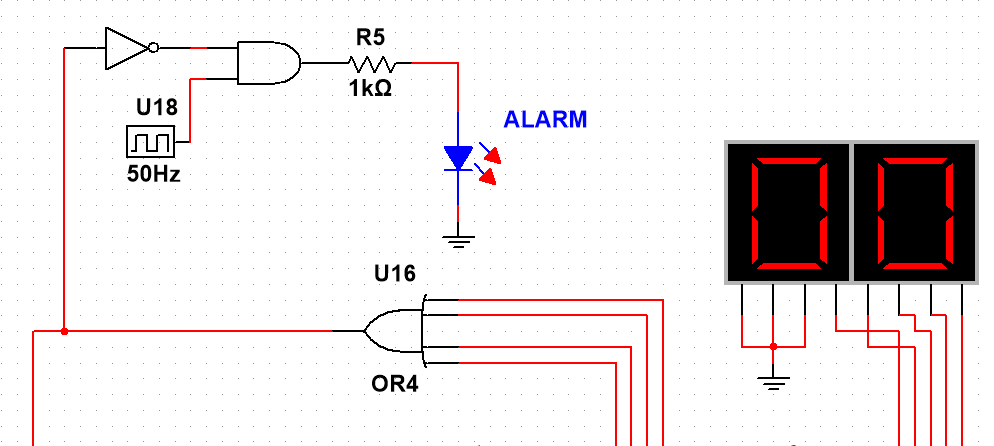
\includegraphics[scale=0.4]{images/alarm}
        \caption{Schemat alarmu}
    \end{figure}

    \section{Pełny układ}
    \begin{figure}[H]
        \centering
        \captionsetup{font=small, skip=2pt}
        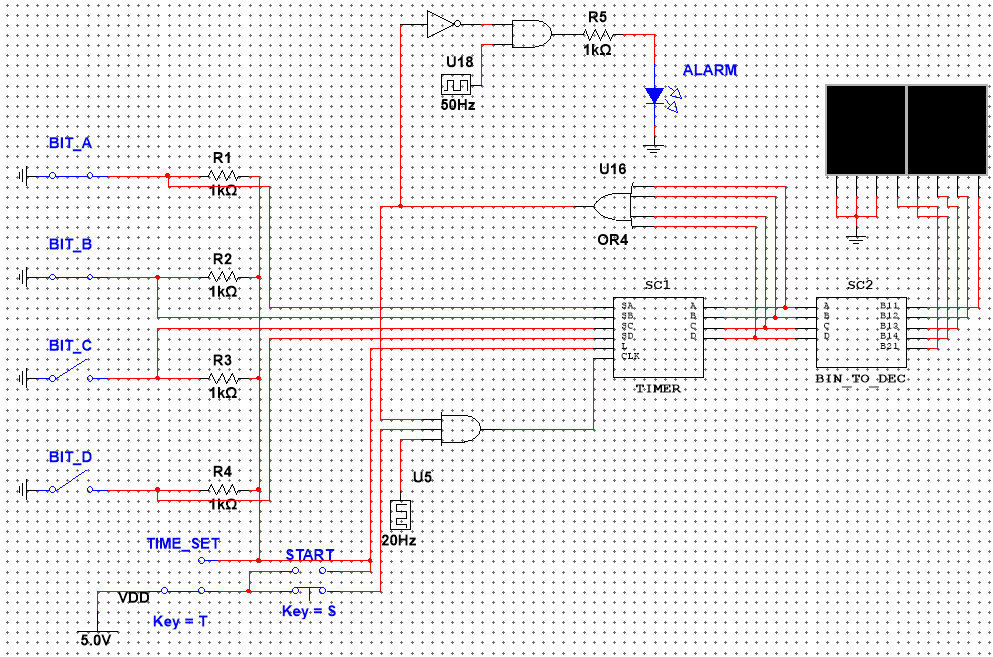
\includegraphics[scale=0.7]{images/pelny_timer}
        \caption{Schemat pełnego układu TIMER w Multisim}
    \end{figure}

    \section{Testowanie}

    \subsection{Testowanie transkodera liczb szesnastkowych na dziesiętne}
    Poniżej został przedstawiony generator liczb od 0 do 15 włącznie zapisane w systemie binarnym,
    które mają zostać przetranskodowane na liczby w systemie dziesiętnym.
    \begin{figure}[H]
        \centering
        \captionsetup{font=small, skip=2pt}
        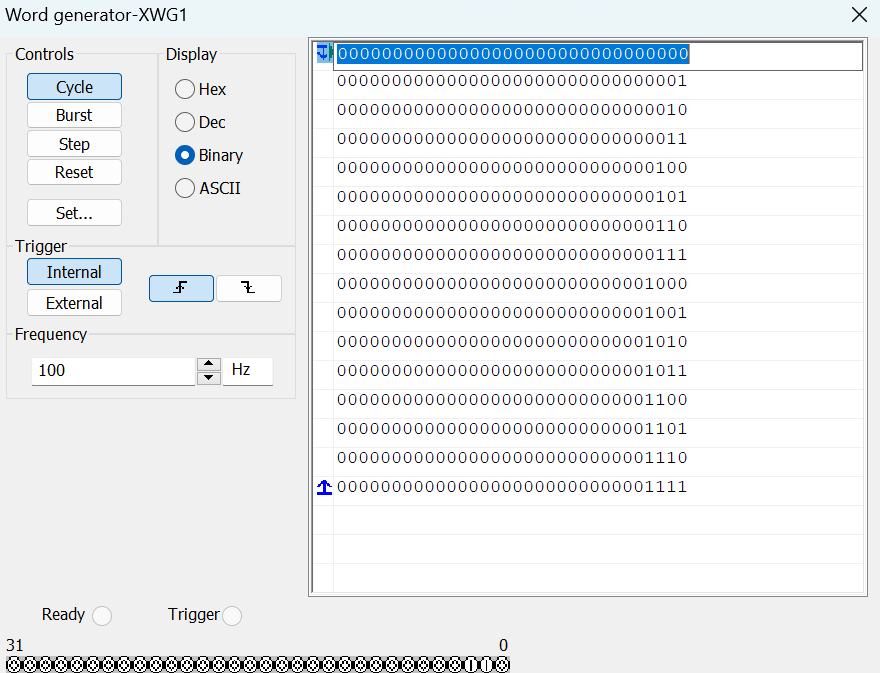
\includegraphics[scale=0.7]{images/generator1}
        \caption{Generator liczb od 0 do 15 włącznie w systemie binarnym}
    \end{figure}
    
    W poniższym generatorze są ustawione oczekiwane wyniki transkodowania liczb.
    \begin{figure}[H]
        \centering
        \captionsetup{font=small, skip=2pt}
        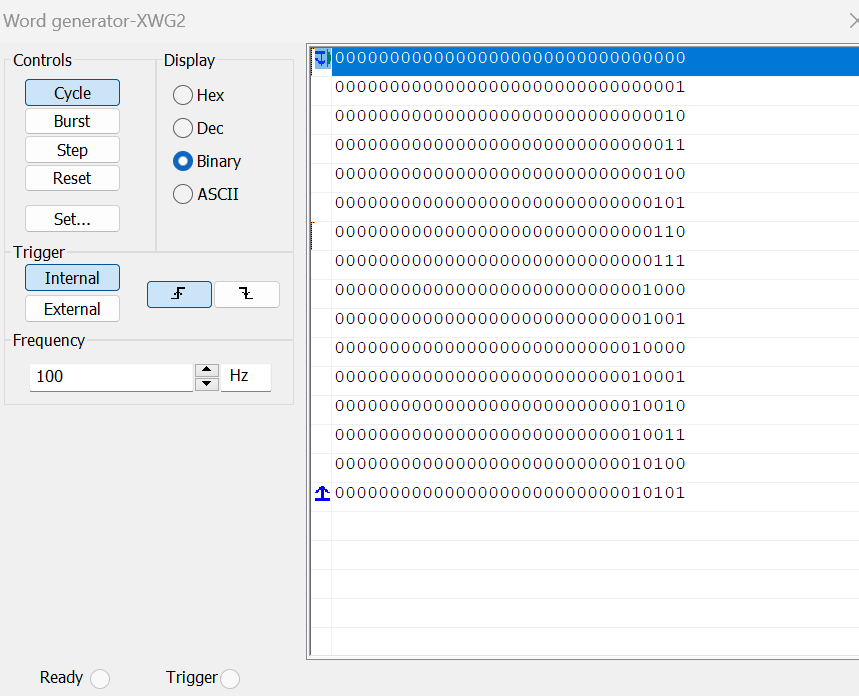
\includegraphics[scale=0.7]{images/generator2}
        \caption{Generator poprawnych kodów liczb w systemie dziesiętnym}
    \end{figure}

    \begin{figure}[H]
        \centering
        \captionsetup{font=small, skip=2pt}
        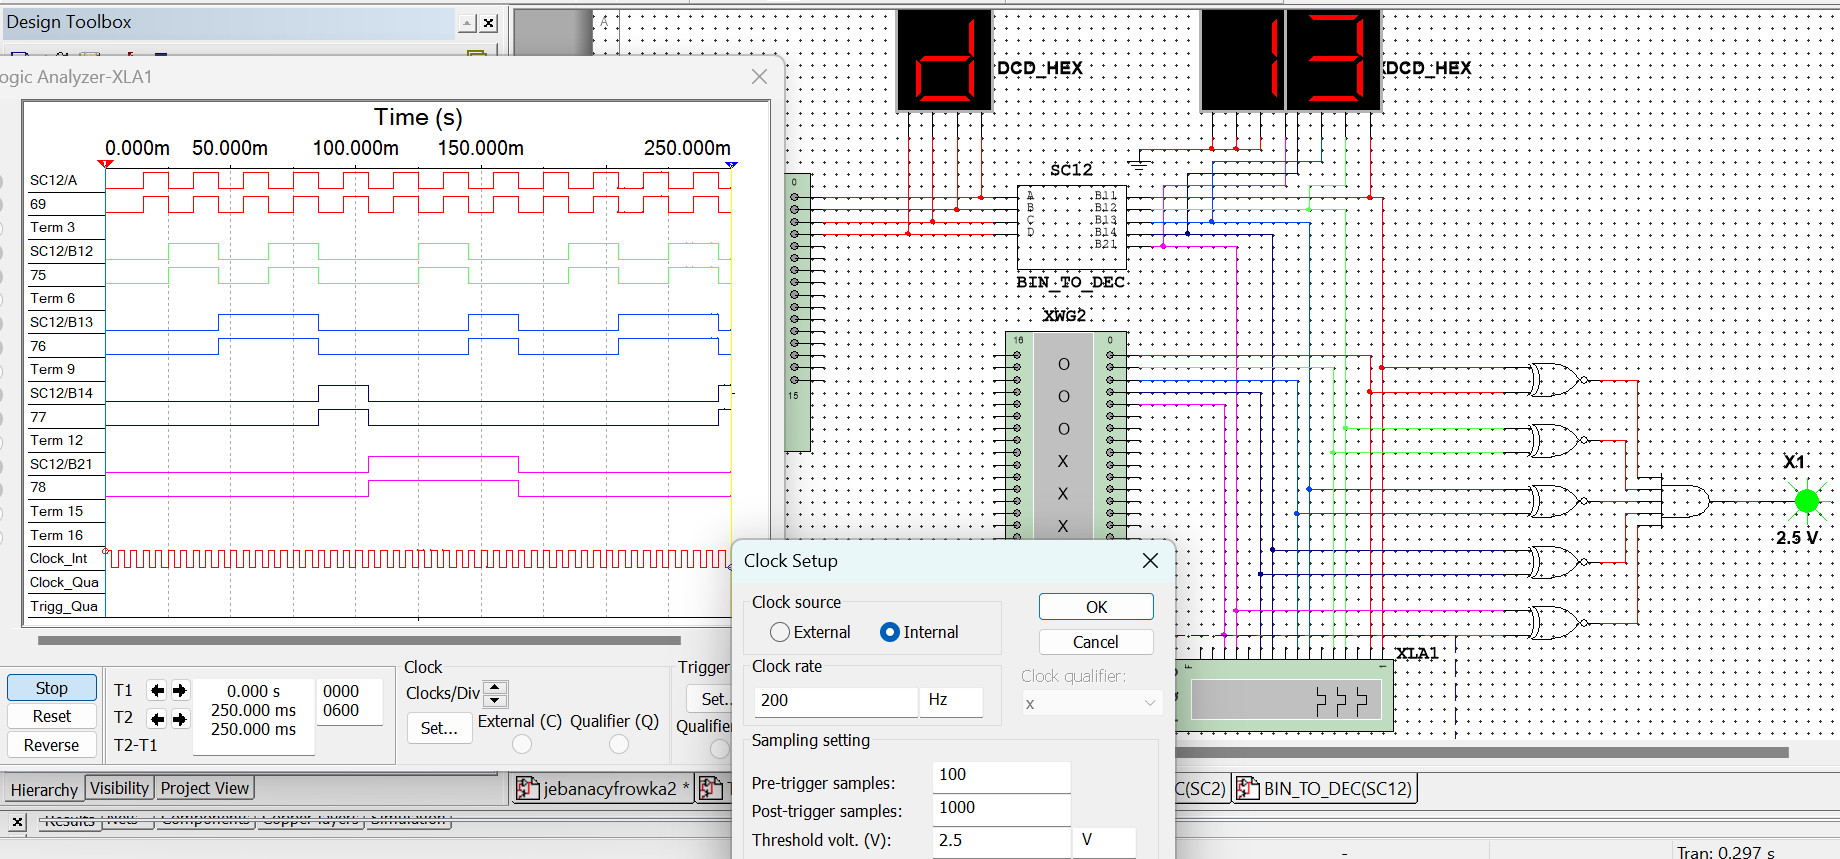
\includegraphics[scale=0.5]{images/analizator_test}
        \caption{Analizator stanów logicznych w układzie testującym}
    \end{figure}
    Z powyższego analizatora widać, że wszystkie sygnały o jednakowych kolorach (za wyjątkiem rzecz jasna
    wewnętrznego sygnału zegarowego analizatora na dole) mają takie same wykresy. 

    \section{Wnioski}
    
    \subsection*{Co można było zrobić lepiej?}
    \begin{itemize}
        \item Użyć licznika synchronicznego
    \end{itemize}

    \section{Zastosowania}

    \begin{itemize}
        \item System informujący o długim czasie otwarcia lodówki \begin{figure}[H]
            \centering
            \captionsetup{font=small, skip=2pt}
            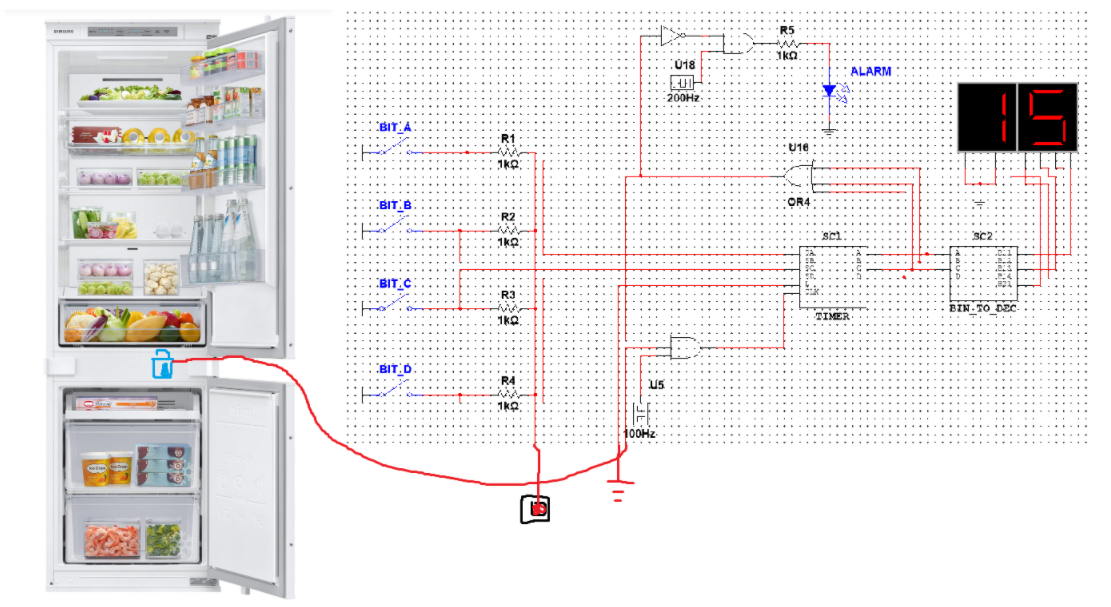
\includegraphics[scale=0.7]{images/lodowka}
            \caption{Zastosowanie układu do informacji o długim otwarciu lodówki}
        \end{figure}
        \item System blokujący drzwi wejściowe do budynku po otwarciu ich przez mieszkańca za pomocą domofonu
        \begin{figure}[H]
            \centering
            \captionsetup{font=small, skip=2pt}
            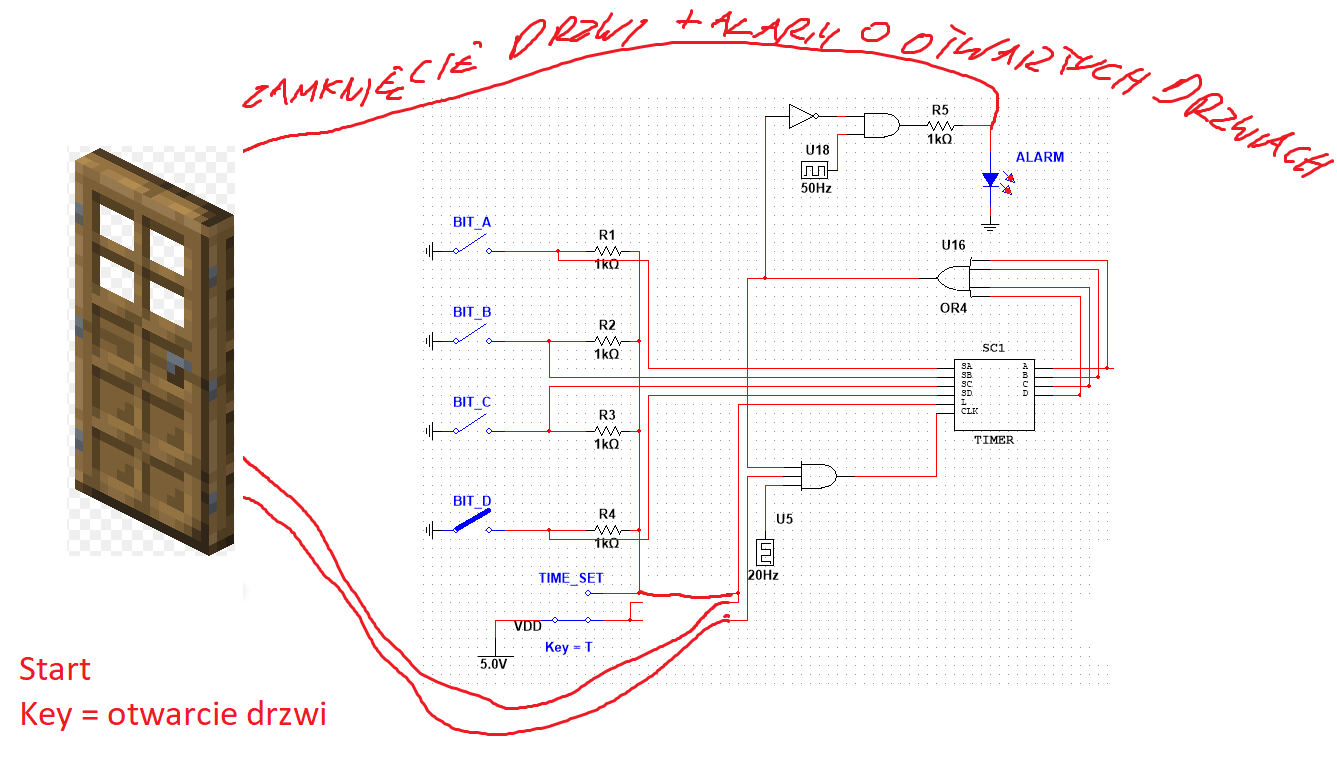
\includegraphics[scale=0.3]{images/drzwi}
            \caption{System blokujący drzwi}
        \end{figure}
        \item Odliczanie czasu do eksplozji bomby \begin{figure}[H]
            \centering
            \captionsetup{font=small, skip=2pt}
            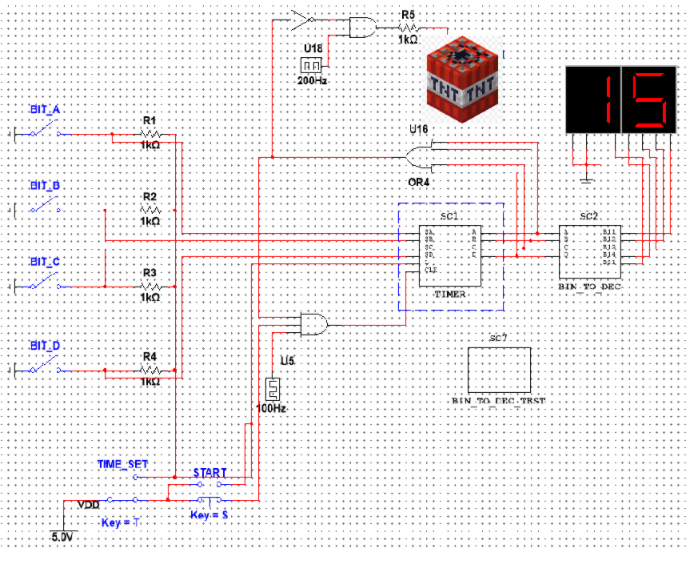
\includegraphics{images/bomba}
            \caption{Odliczanie do eksplozji bomby}
        \end{figure}
    \end{itemize}
    
    
\end{document}